\section{Introduction}

This document describes the problem addressed by mARGOt and it shows how the framework aims at solving it, highlighting the boundaries between what is expected as input and what is the produced output.
Moreover, this guide will describe the framework interface exposed to the user and how to integrate mARGOt in the target application.
This document aims at providing the ``big picture'' of the framework, for implementation details refers to doxygen documentation.

Together with the autotuning framework, it is possible to use an utility, named \textit{mARGOt heel}, which generates an high level interface, hiding as much as possible the implementation details of the integration process.
However, the latter is considered out of scope from this document.


\subsection{Target problem}


The source code describes the functional behavior of the application and it might be abstracted as a function that produces the desired output, starting from an initial input, i.e. $o = f(i)$.
A large class of application might expose software knobs which alter its behavior, i.e.  $o = f(i,k_1,k_2,\ldots,k_n)$.
The idea is that a change on the configuration of those knobs, alter the extra-functional properties (EFP) of the function $f$ (e.g. the execution time or the power consumption) and of the output (e.g. result accuracy or size).

While the functional behavior of the application is utterly described in the source code, its extra-functional behavior is more subtle, since it usually depends on the underlying architecture, on the system workload, on the assigned computational resources and on the current input.
Since the user typically has requirement on the application EFP, selecting the most suitable configuration of the software knobs is not a trivial task.
Moreover, since the system workload, the assigned resources and the input may change at runtime, choosing a one-fits-all configuration may lead to a sub-optimal solution.

In the context of autonomic computing, an application is seen as an autonomous element, which is able to automatically adapt.
The mARGOt autotuning framework aims at enhancing the target application with a runtime adaptation layer, to continuously provide the most suitable configuration according to application requirements and to observation of its actual EFP.


\subsection{Framework overview}

The main idea behind mARGOt is the MAPE\footnote{Kephart, Jeffrey O., and David M. Chess. ``The vision of autonomic computing.'' Computer 36.1 (2003)} loop.
In this context, an autonomic manager is in charge to manage the application, implementing a loop composed by five elements.
The \textbf{M}onitor element provides the ability to gather insight on the actual application behavior, the \textbf{A}nalyse element extract information useful for the \textbf{P}lan element, which select the action actuated by the \textbf{E}xecute element.
The effect of the selected action will be observed by the monitor element, which close the loop.
The fifth element of the MAPE loop is the application knoledge, which is leveraged by all the other elements.

The mARGOt framework is an implementation of the MAPE loop, which focus on providing to the application the self-optimization property.
To improve the versatility of the framework, the Execute element is not part of the framework, but it is the application that is in charge of actuating the action.
In particular, if we model the application as $o = f(i,k_1,k_2,\ldots,k_n)$, mARGOt will provide to the application the most suitable values of the software knobs (i.e. $k_1,k_2,\ldots,k_n$).
For example, if one knob of the application is the number of threads, mARGOt provides the most suitable number of threads, but it is the application in charge of actually spawn or join threads.
This decision, enables the autotuning framework to be agnostic with respect to the nature of the software knobs.


\begin{figure}
	\centering
	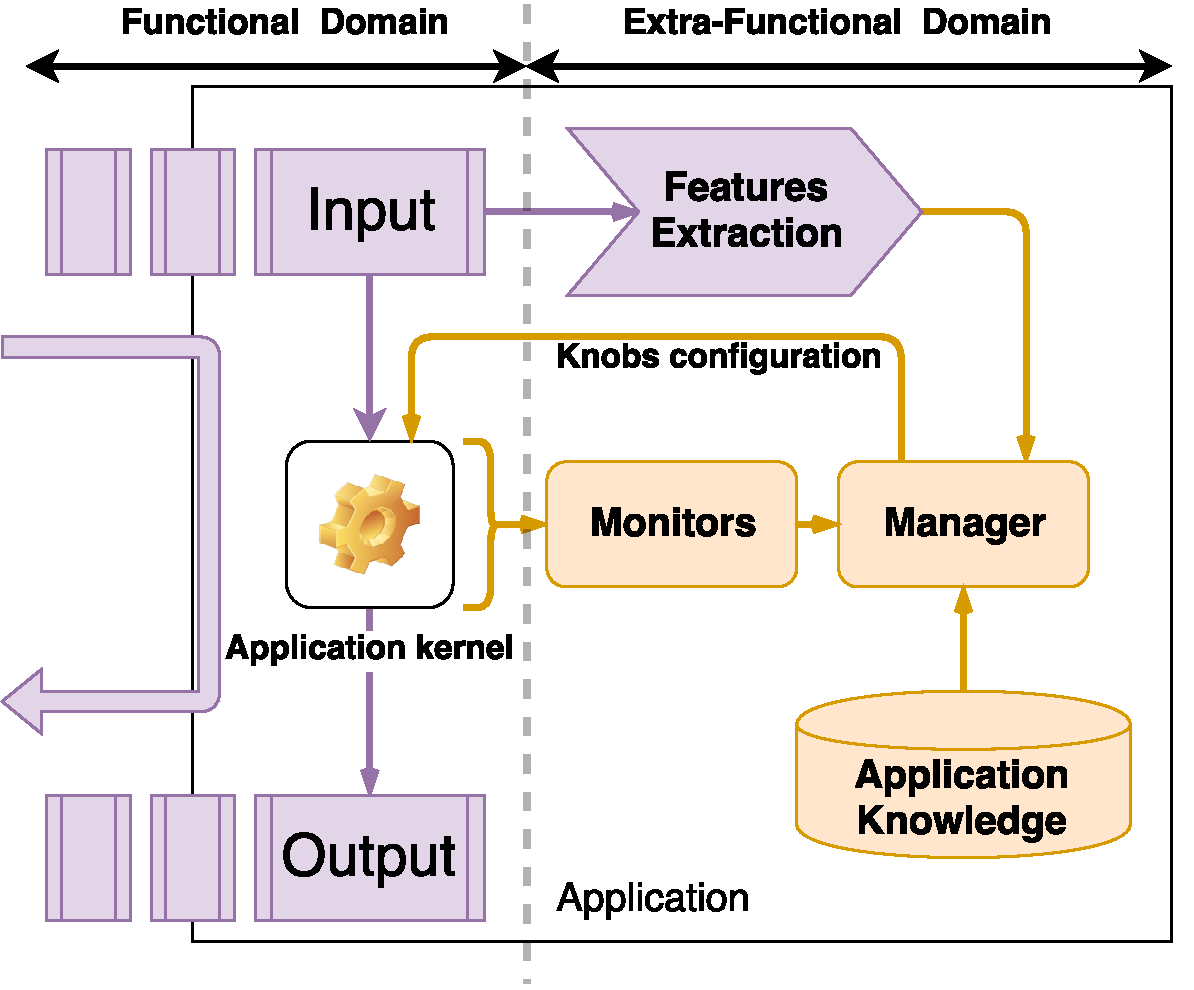
\includegraphics[scale=0.5]{margot_architecture}
	\caption{High level overview of the mARGOt structure (highlighted in orange). Purple elements, represents application code. }
	\label{fig:framework_overview}
\end{figure}


Assuming that the target application is composed by one kernel which elaborate an input to produce an output, \prettyref{fig:framework_overview} shows an overview of the framework structure.
In particular, mARGOt is a C++ library which is linked against the target application.
Therefore, each instance of the application is able to take autonomous decisions.
All the source code that the developer wrote, represented by purple elements, mainly describes the functional domain of the application, i.e. how to produce the output from given the actual input.
All the main modules which compose the autotuning framework, represented by orange elements, aims at tuning dynamically the application kernel according to Extra-Functional requirements and they are mostly orthogonal with respect to the functional aspects.
The only shared region between the user code and the autotuning framework is in charge of extracting features of the input (if any), which might be leveraged by the autotuning to select the most suitable configuration.


The autotuning framework is composed by three modules. 
Obviously, the Monitors module is in charge of acquiring insight on the actual behavior of the application, representing the monitor element of the MAPE loop.
The Manager module represents the analyze and plan elements of the MAPE loop, to provide to the application the most suitable configuration according to the monitor information, the application knowledge, the features of the current input and the user requirements.
The application knowledge is an abstraction of the extra-functional behavior of the application, gathered at design-time through a Design Space Exploration.
However, it is possible to change the application knowledge at runtime.


\subsection{Framework integration}

The purpose of this document is to describe how it is possible to integrate the mARGOt framework in the target application.
Following sections of this document will describe in details the interface and purpose of the monitors, the manger and the application knowledge.
Finally,  \prettyref{sec:integration} will provide an example of integration in a toy application.





